\documentclass[14pt,a4paper]{extarticle}

% ==========================================
% 1. PAQUETES BÁSICOS (Base Principal)
% ==========================================
\usepackage[utf8]{inputenc}
\usepackage[T1]{fontenc}
\usepackage[spanish,es-nodecimaldot]{babel}

% ==========================================
% 2. GEOMETRÍA Y MÁRGENES (Base Principal)
% ==========================================
\usepackage{geometry}
\geometry{top=3cm, bottom=3cm, left=2.5cm, right=2.5cm}

% ==========================================
% 3. GRÁFICOS Y COLORES (Combinado)
% ==========================================
\usepackage{graphicx,epsfig}
\graphicspath{{./resources/imagenes/}} % Carpeta por defecto para imágenes del Doc 2

% Colores (Debe cargarse antes que las cajas)
\usepackage[dvipsnames]{xcolor}
\definecolor{bibi}{RGB}{0,103,148}

% ==========================================
% 4. MATEMÁTICAS Y SÍMBOLOS (Del Doc 2)
% ==========================================
\usepackage{amsmath}
\usepackage{amssymb}
\usepackage{amsthm}
\usepackage{cancel}
\usepackage{dsfont}
\usepackage{wasysym} % (De tu base principal, necesario para \checked y \XBox)
\renewcommand{\proofname}{Demostración}

% ==========================================
% 5. TABLAS, LISTAS Y FORMATO (Combinado)
% ==========================================
\usepackage{titlesec} % (Base Principal)
\usepackage[shortlabels]{enumitem} % Combinado con la opción del Doc 2
\usepackage{booktabs}
\usepackage{tabularx}
\usepackage{longtable}
\usepackage{multicol}
\usepackage{setspace}
\usepackage{verbatim}
\setlength{\parindent}{0pt} % Sangría en cero (Del Doc 2)

% ==========================================
% 6. FLOTANTES, ÍNDICES Y BIBLIOGRAFÍA (Del Doc 2)
% ==========================================
\usepackage{float} 
\usepackage{caption}
\usepackage{subcaption}
\usepackage{tocloft}
\usepackage[numbers]{natbib}

% ==========================================
% 7. ENCABEZADOS Y PIES DE PÁGINA (Del Doc 2)
% ==========================================
\usepackage{fancyhdr}
\usepackage{lastpage}

% ==========================================
% 8. DIAGRAMAS Y ALGORITMOS (Del Doc 2)
% ==========================================
\usepackage{venndiagram}
\usepackage{tikz}
\usetikzlibrary{shapes.geometric}
\usepackage{algorithm}
\usepackage{algpseudocode}

% ==========================================
% 9. CAJAS PERSONALIZADAS (Del Doc 2)
% ==========================================
\usepackage[most]{tcolorbox}

% Caja para Análisis de Juego
\newtcolorbox{analisisbox}[1]{
    colback=bibi!5!white,
    colframe=bibi,
    title=\textbf{#1},
    fonttitle=\bfseries,
    arc=3pt,
    outer arc=3pt,
    boxrule=1pt,
    enhanced,
    drop shadow
}

% Cajas para pros y contras
\newtcolorbox{positiveside}{
    colback=green!5!white,
    colframe=green!50!black,
    title=\textbf{Puntos Positivos \checked},
    fonttitle=\bfseries
}

\newtcolorbox{negativeside}{
    colback=red!5!white,
    colframe=red!50!black,
    title=\textbf{Puntos Negativos \XBox},
    fonttitle=\bfseries
}

% ==========================================
% 10. ENLACES E HIPERVÍNCULOS (Al final siempre)
% ==========================================
\usepackage{hyperref}
\hypersetup{
    colorlinks=true,
    linkcolor=blue,
    filecolor=magenta,      
    urlcolor=cyan,
    citecolor=red, % Extraído del Doc 2
}

% --- ESTRUCTURA DEL DOCUMENTO (Base Principal) ---

\begin{document}

\begin{titlepage}
	\thispagestyle{empty}
	\begin{minipage}[c][0.17\textheight][c]{0.25\textwidth}
		\begin{center}
			
\includegraphics[width=3.5cm, height=3.5cm]{resources/imagenes/Logo_UNAM.png}
		\end{center}
	\end{minipage}
	\begin{minipage}[c][0.195\textheight][t]{0.75\textwidth}
		\begin{center}
			\vspace{0.3cm}
			\textsc{\large Universidad Nacional Aut\'onoma de M\'exico}\\[0.5cm]
			\vspace{0.3cm}
			\hrule height2.5pt
			\vspace{.2cm}
			\hrule height1pt
			\vspace{.8cm}
			\textsc{Facultad de Ciencias}\\[0.5cm] %
		\end{center}
	\end{minipage}
	
	\begin{minipage}[c][0.81\textheight][t]{0.25\textwidth}
		\vspace*{5mm}
		\begin{center}
			\hskip2.0mm
			\vrule width1pt height13cm 
			\vspace{5mm}
			\hskip2pt
			\vrule width2.5pt height13cm
			\hskip2mm
			\vrule width1pt height13cm \\
			\vspace{5mm}
			
\includegraphics[height=4.0cm]{resources/imagenes/Logo_FC.png}
		\end{center}
	\end{minipage}
	\begin{minipage}[c][0.81\textheight][t]{0.75\textwidth}
		\begin{center}
			\vspace{1cm}
			
			{\large\scshape Diseño y Programación de Videojuegos - 7135}\\[.2in]
			
			\vspace{2cm}            
			
			\textsc{\Large \textbf{T}\hspace{0.3cm}\textbf{e}\hspace{0.3cm}\textbf{r}\hspace{0.3cm}\textbf{c}\hspace{0.3cm}\textbf{e}\hspace{0.3cm}\textbf{r}\hspace{0.5cm}\textbf{P}\hspace{0.3cm}\textbf{r}\hspace{0.3cm}\textbf{o}\hspace{0.3cm}\textbf{t}\hspace{0.3cm}\textbf{o}\hspace{0.3cm}\textbf{t}\hspace{0.3cm}\textbf{i}\hspace{0.3cm}\textbf{p}\hspace{0.3cm}\textbf{o}}\\ [2cm]

            
			\textsc{\Large{Alumno:  }\normalsize \\
                \vspace{.3cm}
				\textbf{ 
                \vspace{.2cm}
				Castillo Hernández Antonio - 320017438 \\
				\phone\phone\phone\\
				Lopez Garcia Francisco Daniel - 320104321\\
				\phone\phone\phone\\
				Luna Campos Emiliano - 320292084\\
				\phone\phone\phone\\
                \vspace{1cm}
                  }}    
			
			\textsc{{Fecha de entrega: \\ \textbf{26 de marzo del 2026}}}\\[1.2cm]        
			
			\textsc{{Profesor: \\ \textbf{Enrique Ehecatl Hernández Ferreiro}}}\\[1.2cm]  
			
			\textsc{Ayudantes: \\ \textbf{Joel Haidd Reyes Cedillo \\ Jesús Haans López Hérnandez } }
			
			
			\vspace{0.5cm}
		\end{center}
	\end{minipage}
\end{titlepage}


\newpage
\tableofcontents
\newpage

% --- Contenido ---

\section{The Tower Of Demon´s}
\textsf{The Tower Of Demon´s} es un juego RPG de exploracion de mazmorras, inspirado en juegos como \textsf{The Legend of Zelda} o \textsf{Mario \& Luigi: Superstar Saga} donde los jugadores tendran que ir avanzando entre salas para ascender por los pisos de la torra y al llegar a la cima derrotar al \textsf{Rey demonio}. \\


\section{Descripción General del Juego}
El juego está planificado para superar los cinco pisos de la torre de los sueños y alcanzar la cima donde se encuentra el malvado y misterioso al que muchos llaman \textsf{Rey demonio}. \\

En cada piso, el jugador tiene que explorar las distintas salas para encontrar al guardián de la llave, enemigo que debe ser enfrentado y derrotado, ya que al lograrlo, el jugador obtiene la llave que le permitirá subir al siguiente piso y lograr el gran objetivo. \\

Sin embargo, el trayecto no sera sencillo debido a las peligrosas criaturas que han infestado toda la torre y, debido a su naturaleza despiadada, buscan interponerse en el camino de los jugadores. \\

Para enfrentar a los distintos enemigos, los jugadores tienen la posibilidad de tener distintas variables de combates, como la clase y las posiciones, además de que habrá un sistema de quicktime events al momento de atacar y esquivar para hacer más dinámicos los combates. \\

\section{Experiencia a Transmitir}

En este juego lo que buscamos transmitir es que los jugadores experimenten la curiosidad de explorar las distintas salas para encontrar la llave. \\

Además, queremos que los jugadores resuelvan pequeños problemas en los distintos pisos, como salas bloqueadas en donde los jugadores tendrán que conseguir objetos específicos para avanzar. \\

También buscamos un desafío interesante durante los combates; durante el juego queremos dejar un poco de lado la poca interacción en los combates de un juego RPG clásico en donde solo le dices a tu personaje que ataque y este lo hace de forma automática. En este juego los jugadores tendrán que presionar una combinación de teclas del teclado para poder atacar, haciendo una experiencia más inmersiva, metiendo más al jugador al combate. \\

Es decir, el juego está pensado para combinar elementos tradicionales del género RPG con sistemas de interacción activa que vuelven el combate más inmersivo y desafiante. \\

Y para los jugadores más osados y técnicos, el juego ofrece un sistema de debilidades dobles para que los jugadores formen las mejores estrategias para derrotar a los guardianes. \\

\subsection{Objetivos}
\begin{itemize}
    \item \textbf{Objetivo Principal:} El objetivo principal del juego es llegar al ultimo piso de la torre en donde se encuentra el Rey demonio y derrotarlo.
    \item \textbf{Objetivos Secundarios:} Maxear el nivel de los heroes y hacer la mejor build.
\end{itemize}

\section{Mecánicas y Recursos}
\subsection{Recursos del Juego}
\begin{itemize}
    \item \textbf{Héroes:} Durante los combates, el jugador podrá controlar a tres héroes, los cuales podrá mejorar con objetos y subiéndolos de nivel. Cada héroe tiene una clase distinta, así que el jugador tiene que gestionar qué héroe usará para atacar a un enemigo en específico.
    
    \item \textbf{Vida:} Los tres héroes tendrán una barra de vida, la cual bajará si reciben un ataque enemigo, siendo que también pueden recuperarla con objetos o bebiendo de la fuente.

    \item \textbf{Energía:} Los tres héroes tendrán una barra de energía, la cual se consumirá si el   jugador elige hacer un ataque especial; esta barra podrá regenerarse mediante el uso de objetos o bebiendo de la fuente.

    \item \textbf{Experiencia:} Al terminar un combate, los héroes obtendrán puntos de experiencia, los cuales, al obtener los suficientes, estos subirán de nivel.

    \item \textbf{Doblones:} Estos objetos son la moneda del juego y se podrán usar para comprar objetos y armas en la tienda; además, al terminar un combate, el jugador recibirá cierto número de doblones; también se pueden conseguir al abrir cofres.

    \item \textbf{Objetos:} Los jugadores podrán obtener objetos mediante cofres o comprándolos en la tienda; estos tendrán distintos usos para ayudar en la aventura.

    \item \textbf{Orbe de posición:} Este objeto especial permitirá a los jugadores cambiar la posición de los héroes a cambio de consumirlo; este podrá conseguirse en la tienda, además de que al iniciar la aventura el jugador contará con 3 orbes.

    \item \textbf{Armas:} Estos objetos aumentarán las estadísticas base de los héroes, las armas podrán conseguirse en la tienda o en cofres.

    \item \textbf{Llaves:} Este objeto se usará para poder abrir la puerta hacia el siguiente piso, gastándose en el proceso, y se obtiene al derrotar al guardián del respectivo piso.

    \item \textbf{Objetos clave:} En los distintos pisos habrá objetos clave que le permitirán al jugador avanzar por salas que están bloqueadas; los objetos clave estarán de forma permanente en el inventario para poder usarse en los distintos pisos. Estos objetos estarán protegidos por enemigos, así que habrá que derrotarlos para obtener el objeto.

    \item \textbf{Cofres:} Por las distintas salas, el jugador podrá encontrar cofres que, al abrirlos, podrá obtener monedas, objetos o armas; una vez abiertos, los cofres estarán vacíos.

    \item \textbf{Turnos:} Los combates estarán divididos en turnos; el jugador deberá administrar bien sus turnos para poder terminar el combate de forma eficiente.

    \item \textbf{Tiempo/Combates:} El tiempo del juego se mide en combates, cuando la fuente se seca o la tienda cierra el jugador tendra que tener 3 combates para que el tiempo pase y la fuente tenga agua y la tienda abra de nuevo.

    \item \textbf{Fuente de los Sueños:} Una maravillosa fuente que se encuentra en la sala inicial de cada piso; esta permitirá guardar la partida, además de curar al equipo  y recuperar su energia bebiendo del agua. Al beber del agua, la fuente se secará y tendrás que disputar tres combates para que el agua fluya de nuevo.
\end{itemize}

\section{Reglas del Sistema}
\subsection{Reglas del piso}
\begin{itemize}
\item En cada piso, el jugador comienza en una sala inicial.
\item En la sala inicial no aparecen enemigos.
\item En la sala inicial siempre hay una fuente de los sueños y una tienda.
\item Al entrar por primera vez a la sala inicial, el agua de la fuente se restaura y la tienda hace restock de objetos.
\item Al derrotar a un enemigo, este reaparece después de 3 minutos.
\item No puedes obtener la llave sin haber derrotado antes al guardián del piso.
\item El unico enemigo en la sala del guardian es el propio guardian.
\item Al abrir la puerta al siguiente piso, la llave se gasta y se pierde.
\item Al subir un piso, el jugador no podrá descender al anterior.
\item Si te acercas mucho a los enemigos, estos comenzarán a perseguirte.
\item Al entrar en contacto con un enemigo, se entrará en modo combate.
\end{itemize}

\subsection{Reglas del combate}
\begin{itemize}
\item El combate dara inicio hasta que el jugador cambia la posicion de los heroes o si decide no hacer cambios. 
\item En dado caso de no contar con orbes de posicion el combate dara inicio directamente.
\item El orden de los turnos de los heroes y los enemigos es decidido por quien tiene mayor velociad.
\item El combate terminara si el jugador logra derrotar a todos los enemigos o si todos los heores son derrotados.
\item Al terminar el combate el jugador recibira cierto numero de monedas y puntos de experiencia.
\item Cada uno de los heroes podra realizar una accion por turno, ya sea atacar, defenderse o usar un objeto.
\item Si el jugador falla mas de la mitad de la secuencia de teclas al atacar, el ataque falla.
\item Si el jugador falla menos de la mitad de la secuencia de teclas al atacar, el ataque hace la mitad del daño.
\item Si el jugador realiza correctamente la secuenca de teclas el daño del ataque no se ve alterado.
\item Si el nivel del heroe es menor al del enemigo que lo ataca este no tendra la oportunidad de esquivar.
\item Si el jugador falla al presionar la tecla de esquive recibira el daño del ataque enemigo.
\item Cuando el guardian tenga menos del \%50 de su vida llamara a dos aliados para que lo ayuden.
\end{itemize}

\subsection{Reglas de las armas}
\begin{itemize}
\item Sieg solo puede equiparse armas de Melee (Espadas).
\item Merlin solo puede equiparse armas de Rango (Baculos).
\item Heracles solo puede equiparse armas de Tanque (Escudos).
\item Al inicio del juego los tres heroes comienzan con armas basicas equipadas.
\item Los heroes solo pueden tener equipada un arma a la vez
\end{itemize}

\subsection{Reglas de clases}
\begin{itemize}
\item Si un personaje de clase Melee ataca a uno de clase Rango el daño de ataque aumenta un \%50, por el contrario si a ataca a uno de clase Tanque el daño de ataque se reduce un \%50.
\item Si un personaje de clase Rango ataca a uno de clase Tanque el daño de ataque aumenta un \%50, por el contrario si ataca a uno de clase Melee el daño de ataque se reduce un \%50
\item Si un personaje de clase Tanque ataca a uno de clase Melee el daño de ataque aumenta un \%50, por el contrario si ataca a uno de clase Rango el daño de ataque se reduce un \%50
\end{itemize}

\subsection{Reglas de posicion}
\begin{itemize}
\item Si un personaje de posicon en tierra ataca a uno de posicion bajo tierra el daño de ataque aumenta un \%50, por el contrario si a ataca a uno de posicion volando el daño de ataque se reduce un \%50.
\item Si un personaje de posicon volando ataca a uno de posicion en tierra el daño de ataque aumenta un \%50, por el contrario si a ataca a uno de posicion bajo tierra el daño de ataque se reduce un \%50.
\item Si un personaje de posicon bajo tierra ataca a uno de posicion volando el daño de ataque aumenta un \%50, por el contrario si a ataca a uno de posicion en tierra el daño de ataque se reduce un \%50.
\end{itemize}

\subsection{Reglas de los stats}
\begin{description}
    \item[Salud (HP)] 
        Si la salud llega a 0 el heroe cae derrotado y no puede actuar.
    
    \item[Ataque (ATK)]
        El daño infligido se calcula multiplicando el daño base del ataque por un multiplicador fijo de $1.5$ por cada punto de punto de Ataque.


    \item[Defensa (DEF)]
        Cada punto de defensa aplica un multiplicador de reducción del $0.02$ sobre el daño recibido.

    \item[Energía (EN)]
     Si la barra llega a cero el heroe no podra hacer ataques especiales.

    \item[Maestría (MST)]  
    \begin{itemize}
        \item Reduce el número de teclas en la secuencia en $-1$ por cada 15 puntos de MST.
        \item Incrementa el tiempo del timing en un $5\%$ por cada dos puntos de MST.
    \end{itemize}
\end{description}

\subsection{Reglas de la tienda}
\begin{itemize}
\item El jugador puede comprar hasta 3 unidades de cada objeto.
\item En la tienda siempre se venderan 3 objetos de forma aleatoria.
\item Una vez compras una arma en especifico esta no vuelve a aparecer en la tienda.
\item Los objetos de la tienda se reinician despues de 3 combates.
\item Si compras todos los objetos de la tienda esta se cerrara y no abrira hasta despues de 3 combates.
\end{itemize}

\subsection{Reglas de la fuente}
\begin{itemize}
\item Al beber de la fuente la vida y la energia de los 3 heores se regenera al completo.
\item El beber de la fuente esta se secara y no podras beber de nuevo.
\item El agua de la fuente vuelve a fluir despues de 3 combates.
\item El jugador puede guardar la partida las veces que quiera.
\end{itemize}

\subsection{Reglas generales}
\begin{itemize}
\item Al comenzar una partida nueva el jugador comienza en el piso 0.
\item Si los heroes son derrotados en combate el jugador regresa a la sala incial, los heroes regresan a la vida con un \%25 de su barra de vida y de energia y pierden la mitad de sus monedas.
\item Para completar el juego el jugador debe derrotar al Rey demonio.
\item Al terminar el juego puedes cargar una partida o comenzar una nueva.
\end{itemize}

\section{Personajes y Enemigos}
\subsection{Héroes}

\textbf{Sieg.} Él es un joven de origen humilde bendecido con excelentes habilidades de esgrima. De los tres heores el es el mas equilibrado entre fuerza, velocidad y resistencia.

\begin{itemize}
    \item \textbf{Clase:} Melee
    \item \textbf{Posición:} En tierra (Por defecto)
\end{itemize}

\begin{flushleft}
    
\includegraphics[width=0.3\textwidth]{resources/imagenes/Personajes/Sieg.jpg}
\end{flushleft}

\vspace{1em}

\textbf{Merlin.} Él es alguien muy inteligente y estudioso, posee un gran potencia pero es algo lento y tiene poca resistencia.
\begin{itemize}
    \item \textbf{Clase:} Rango
    \item \textbf{Posición:} En tierra (Por defecto)
\end{itemize}

\begin{flushleft}
    
\includegraphics[width=0.3\textwidth]{resources/imagenes/Personajes/Merlin.jpg}
\end{flushleft}

\vspace{1em}

\textbf{Heracle.} Heracles es el mas fuerte y resistente del grupo por lo que puede levantar escudos pesados,sin embargo, es muy lento.
\begin{itemize}
    \item \textbf{Clase:} Tanque
    \item \textbf{Posición:} En tierra (Por defecto)
\end{itemize}

\begin{flushleft}
    
\includegraphics[width=0.3\textwidth]{resources/imagenes/Personajes/Heracles.jpg}
\end{flushleft}

\subsection{Personajes Aliados}
\textbf{Kafei.} Un hombre lleno de deudas que busco el trabajo más peligroso para conseguir algunos doblones, abrir una tienda en una torre demoniaca.

\begin{flushleft}
    \includegraphics[width=0.3\textwidth]{resources/imagenes/Personajes/Kafei.jpg}
\end{flushleft}

\subsection{Personajes Enemigos}
\textbf{Slime.} Un ser verde y gelatinozo, su fuerza, velocidad o resistencia no son tan destacables,acostumbran a atacar con varios miembros de su especie.
\begin{itemize}
    \item \textbf{Clase:} Melee
    \item \textbf{Posición:} En tierra
\end{itemize}

\begin{flushleft}
    
\includegraphics[width=0.3\textwidth]{resources/imagenes/Personajes/Slime.jpg}
\end{flushleft}

\vspace{1em}

\textbf{Murcielago.} Animal alado corrompido por la magia oscura, es veloz pero su resistencia es baja, esta hacienzo por beber sangre.
\begin{itemize}
    \item \textbf{Clase:} Rango
    \item \textbf{Posición:} Volando
\end{itemize}

\begin{flushleft}
    \includegraphics[width=0.3\textwidth]{resources/imagenes/Personajes/Bat.jpg}
\end{flushleft}

\vspace{1em}

\textbf{Topo.} Animal corrompido por la magia oscura, es lento pero lo compensa con gran fuerza y excelente resistencia, se dice que son capaces de morder hasta el acero mas duro.
\begin{itemize}
    \item \textbf{Clase:} Tanque
    \item \textbf{Posición:} Bajo tierra
\end{itemize}

\begin{flushleft}
    
\includegraphics[width=0.3\textwidth]{resources/imagenes/Personajes/Topo.jpg}
\end{flushleft}

\vspace{1em}

\textbf{Esquleto.} Restos humanos reanimados por la magia oscura, su unico objetivo es acabar con los humanos vivos para quitarles su piel y cubrir sus huesos.
\begin{itemize}
    \item \textbf{Clase:} Melee
    \item \textbf{Posición:} En tierra
\end{itemize}

\begin{flushleft}
    \includegraphics[width=0.3\textwidth]{resources/imagenes/Personajes/Esqueleto.jpg}
\end{flushleft}

\vspace{1em}

\textbf{Nucifera.} Guardian del primer piso de la torre, esta es una flor que fue maldecida por la magia del Rey demonio, tiene una hambre voraz y se comera todo lo que este al alcance de su boca, sus enredaderas cubren todo el primer piso.
\begin{itemize}
    \item \textbf{Clase:} Melee
    \item \textbf{Posición:} En tierra
\end{itemize}

\begin{flushleft}
    
\includegraphics[width=0.3\textwidth]{resources/imagenes/Personajes/Nucifera.jpg}
\end{flushleft}

\vspace{1em}

\textbf{Rey demonio.} Un ser malvado de origen desconocido que ha corrompido la torre de los sueños, esta recuperando su poder para poder conquistar el mundo.


\section{Análisis de Lentes de Diseño}

Los siguiente son los lentes de diseño que parecieron adecuados como guia para el prototipo

\begin{itemize}
    
    \item \textbf{Lente de la fantasia:} El juego ocurre en una torre controlada por un ente demoniaco con esbirros a lo largo de ella. Queriamos proporcionar un universo fantastico y corrompido  por el caos en el cual te conviertas en un heroe medieval que purga la sagrada torre de los sueños de seres oscuros mediante todo tipo de habilidades y poderes. Lo que se busca con el lente es enfocar estas ideas a que se hagan realidad y el jugador de verdad entre en la fantasia de lleno.
    
    \item \textbf{Lente del Canales y Dimensiones:} Al ser un RPG por turnos, es necesario poner en pantalla distintos iconos, las llaves, el mapa, los objetos que se lleven en el inventario. Ademas se debe mostrar la vida de los heroes, los botones de los time quick events. El lente nos ayuda a saber que es lo que debemos de mostrar, donde lo debemos mostrar, que tan grande deben de ser estas señalizaciones entre otras desciciones.
    
    \item \textbf{Lente del Tiempo:} La reaparición de enemigos a los 3 minutos busca generar urgencia durante la exploración. Este lente nos ayuda a evaluar si ese límite de tiempo es justo y si equilibra adecuadamente los momentos de tensión y calma.

    \item \textbf{Lente de la Simplicidad y Complejidad:} El combate incluye múltiples mecánicas. Este lente asegura que esta profundidad genere estrategias intuitivas y gratificantes (complejidad emergente), evitando abrumar al jugador con demasiadas reglas para que sea fácil de entender pero difícil de dominar.
    
    \item \textbf{Lente de la inspiracion:} Este lente se encontro adecuado para explorar distintas experiencias que tengamos, desde el tipo de juego que elegimos, la estetica, las mecanicas. Tuvimos las distintas ideas y las juntamos en un juego inspirado en experiencias como pokemon o sea of stars. 
\end{itemize}

\section{Procedimientos y Límites}
\subsection{Procedimientos}
En la pantalla de inicio el jugador puede crear una partida o cargar una ya guardada. \\

Al crear un partida nueva el jugador comenzara en el piso 0, aqui no habra enemigos, solo habran tres personas que le enseñaran al jugador como combatir contra los enemigos. Al terminar el entrenamiento el jugador podra acceder al piso 1. \\

En cada piso el jugador debe explorar las distintas salas hasta hallar al guardian, la sala del guardian estara bloqueada por lo que el jugador necesitara encontrar un objeto clave para abrir la sala del guardia. \\

Al vecer al guardian se pdora obtener la llave y avanzar al siguiente piso. \\

Al iniciar el combate el jugador tendra la opcion de cambiar la posicion de los heroes por cualquiera de las otras dos posciones. \\

El combate se divide en turnos siendo que las unidades mas rapidas actuan antes. \\

Si el jugador decide atacar puede escoger entre un ataque normal (el cual no consume energia) y una especial (el cual tendra un cierto consumo de energia). El jugador tambien podra defenderse para evitar gran parte del daño recibido, si decide usar un objeto lo podra usar en si mismo o en algun aliado pero esto consume un turno. \\



\subsection{Límites}

\begin{itemize}
    \item Solo puede haber un maximo de 5 enemigos por sala. \\

\item El numero maximo de enemigos que enfrentas al mismo tiempo es de 4. \\

\item El jugador solo puede llevar hasta 10 unidades de un mismo objeto. \\

\item El numero maximo de combates en que la fuente esta seca, que la tienda esta cerrada o que la tienda hace un restock es de 3 combates. \\

\item Los heroes y enemigos solo pueden hacer una accion por turno. \\

\item El numero limite de monedas que puede tener el jugador es de 500. \\

\item El numero limite de llaves que puede tener el jugador es de 1. \\

\item El limite de objetos equipables es de 3. \\

\item En cada piso el jugador tendra un limite de nivel maximo:
   \begin{itemize}
    \item Piso 1 nivel maximo 10
    \item Piso 2 nivel maximo 20
    \item Piso 3 nivel maximo 30
    \item Piso 4 nivel maximo 40
    \item Piso 5 nivel maximo 50
    \end{itemize}

\item El limite de los stats es el siguiente:
   \begin{itemize}
    \item El limite de salud es de 500 puntos.
    \item El limite de ataque es de 200 puntos.
    \item El limite de defensa es de 200 puntos.
    \item El limite de velocidad es de 200 puntos.
    \item El limite de energia es de 300 puntos.
    \item El limite de maestria es de 120 puntos.
    \end{itemize}

\end{itemize}



\section{Conflicto y Resultados}

\subsection{Conflictos}
En el camino hacia la cima habra varios enemgios que le impidan el paso a los heroes, tambien habra salas bloqueadas que dificultaran el camino. \\

Los guardianes del piso tambien sera un obstaculo que los heroes deben enfrentar. \\

Al final del juego los heroes tendran que decidir que hacer con el corazon del Rey demonio, ¿comerlo o destruirlo? \\

\subsection{Resultados}
El objetos de los heroes es ascender a la torre y derrotar al Rey demonio, si el jugador logra derrotarlo el jugador podra conseguir dos finales:

\begin{itemize}
    \item \textbf{Final Bueno}: Si los heroes destruyen el corazon del Rey demonio habran liberado a la torre de los sueños de su maldicion.
    \item \textbf{Final Malo}: Si el corazon no es destruido Sieg se vera tentado por el poder, consumira el corazon y se convertira en el nuevo Rey demonio asesinando a sus compañeros en el proceso.
\end{itemize}

Si el jugador es derrotado en combate aparecera una pantalla de Game Over y le dara la opcion de continuar la partida o ir al menu.

\section{Narrativa}

Hace milenios, un monarca cegado por la ambición buscó someter al mundo bajo su poder. Para lograrlo, convocó a los magos más poderosos de su era, quienes, mediante rituales prohibidos, atrajeron a este plano una reliquia de maldad pura conocida como el \textbf{Corazón de la Oscuridad}. Antes de que el rey pudiera consumir el Corazón, fue derrocado por una rebelión; el nuevo linaje real, consciente del peligro y siendo incapaces de destruirlo, decidió sellar el Corazón en lo profundo de la \textit{Torre de los Sueños}. Esta estructura era un regalo divino que albergaba la Fuente de los Sueños, cuyas aguas eran capaces de sanar cualquier mal y preservar instantes en el tiempo. \\

El sello permaneció intacto durante eones, hasta que el paso del tiempo y la negligencia en la vigilancia y mantenimiento de la Torre debilitaron el sello magico. En un giro trágico del destino, una criatura incocente, una cabra que se coló en el recinto sagrado devoró el Corazón, transformándose instantáneamente en el \textbf{Rey Demonio}. Tras consumir la pureza de la Fuente y corromper la Torre con magia oscura, el nuevo soberano del mal lanzó una sentencia sobre la humanidad: \\

\begin{quote}
    \textit{En un año, mi poder se restaurará por completo y el mundo quedará sumergido en la oscuridad eterna.}
\end{quote}

Ante la inminente aniquilación, los reyes más grandes unieron sus voluntades para ejecutar un antiguo hechizo capaz de hallar a los humanos más aptos para la batalla. Así fueron elegidos los tres salvadores: \textbf{Sieg}, un talentoso espadachín de origen humilde; \textbf{Merlín}, un prodigio de la Academia de Magia; y \textbf{Heracles}, el hombre poseedor de la fuerza física más devastadora de la historia. Juntos, los tres héroes se embarcarán en una aventura que decidirá el destino de la humanidad.

\section{Pruebas con usuarios}
\subsection{Hermana de Daniel}

\begin{description}
    \item[Perfil del jugador:] Ella ha jugado algunos juegos sandbox como Minecraft, pero su gran mayoría de juegos son los creados en Roblox.
    
    \item[Descripción de las sesiones de prueba:] Se observó una confusión inicial, peor tras una serie de preguntas de su parte, la jugadora logró entender las reglas del juego.
    
    \item[Hallazgos principales:] No hizo combates mas allá de los necesarios (El del guardian y el combate para liberar las tijeras).
    
    \item[Problemas detectados:] Le costo entender un poco el triangulo de debilidades y fallaba al realizar las secuencias de teclas.
    
    \item[Cambios propuestos al diseño:] Hacer mas fáciles las secuencias de teclas y obligar al jugador a combatir contra los enemigos de las salas.
\end{description}


\subsection{Primo de Emiliano}

\begin{description}
    \item[Perfil del jugador:] Jugador de accion-aventura
    
    \item[Descripción de las sesiones de prueba:] El juego le parecia algo complicado de entender al principio, pero aun asi la idea le parecia buena.
    
    \item[Hallazgos principales:] Le recordo a los juegos de los 90's. Los jefes le parecieron justos y le gusto mucho los time quick events y sintio bien los mensajes que salian de hacerlos perfectos o hacerlos bien
    
    \item[Problemas detectados:] La dinamica de la tienda le parecio engorrosa pero comento que alomejor era por ser fisica. Otro comentario fue la apariencia, que no le terminaba de convencer para la idea que era
    
    \item[Cambios propuestos al diseño:] Mejorar la visualizacion del juego y la interacción con la tienda
\end{description}


\subsection{Primo de Antonio}
\begin{description}
    \item[Perfil del jugador:] Jugador de juegos tipo Shooters
    
    \item[Descripción de las sesiones de prueba:] El juego le parecia algo complicado de entender al principio, pero aun asi la idea le parecia buena.
    
    \item[Hallazgos principales:] Le gusto bastante que existieran clases de jugador y una tienda de items.
    
    \item[Problemas detectados:] A la hora de los combates le costaba un poco  hacer la secuencia de teclas para atacar y el sistema de ataque le parecia un poco conplejo pero despues de 3 intentos le fue agarrando la onda.
    
    \item[Cambios propuestos al diseño:] Tratar de simplificar un poco el sistema de combate.
\end{description}

\section{Cosas que no se pudieron poner en el prototipo}
Debido a las limitaciones de un prototipo hecho con papel hay varias cosas que no pudimos implementar pero que representamos o que directamente no pudimos hacer. \\

Para empezar el prototipo solo representa el primer piso de la torre, hacer los 5 pisos mas el piso 0 del tutorial habria sido una tarea titanica, asi que prefirimos enfocarnos en mostrar un piso de la torre para representar la experiencia que queremos transmitir. \\

La interfaz del invetario y la vista para ver las estadisticas y objetos de los heroes esta ahi pero no son funcionales. \\

El mapa aunque muestra el mapa completo no muestra la ubicacion actual. \\

La tienda solo vende tres objetos, orbes de posicionamiento, pocion de vida y pocion de energia, la tienda real deberia vender eso y más. \\

El sistema de combate hasta eso esta simplificado, el enemigos no tienen una vida real, mas bien somos nosotros los que decidimos cuantos golpes resisiten auntes de caer. \\

La barra de vida y energia de los heroes no se actualizan. \\

Al no poder determinar la velocidad de cada heroes o mosntruos simplificamos el sistema a Los heroes van primero y los monstruos despues. \\

Lo mismo con la maestria, al no poder hacer que esta cambie, se decidio por hacer que las secuencias de teclas sean fijas (en este caso 3 secuencias diferentes). \\

Ademas de que aunque la experiencia de teclear esta, no hay manera de determinar si el usario se equivoca o no al teclear, lo mismo para esquivar. \\

Se omitio el sistema de niveles para enfocarse en el combate. \\


\section{Imagenes del prototipo}
\subsection{Prototipo Físico / Mock-ups}
 \begin{figure}[H]
    \centering
    \includegraphics[width=0.8\textwidth]{resources/imagenes/MockUp/Mapa_Completo.jpg}
    \caption{Imagen del mapa completo}
 \end{figure}


 \begin{figure}[H]
    \centering
    \includegraphics[width=0.8\textwidth]{resources/imagenes/MockUp/Map1.jpg}
    \caption{Imagen de una parte del mapa}
 \end{figure}


 \begin{figure}[H]
    \centering
    \includegraphics[width=0.8\textwidth]{resources/imagenes/MockUp/Map2.jpg}
    \caption{Imagen de una parte del mapa}
 \end{figure}

 \begin{figure}[H]
    \centering
    \includegraphics[width=0.8\textwidth]{resources/imagenes/MockUp/Interfaces.jpg}
    \caption{Imagen de la interfaz de la tienda, mapa y menu.}
 \end{figure}

\begin{figure}[H]
    \centering
    \includegraphics[width=0.8\textwidth]{resources/imagenes/MockUp/ZonaTijeras.jpg}
    \caption{Imagen de la sala donde consigues las tijeras}
 \end{figure}

  \begin{figure}[H]
    \centering
    \includegraphics[width=0.8\textwidth]{resources/imagenes/MockUp/Guardian.jpg}
    \caption{Imagen del Guardian del Piso 1}
 \end{figure}

   \begin{figure}[H]
    \centering
    \includegraphics[width=0.8\textwidth]{resources/imagenes/MockUp/ZonaGuardian.jpg}
    \caption{Imagen de la sala del Guardian del Piso 1}
 \end{figure}

\begin{figure}[H]
    \centering
    \includegraphics[width=0.8\textwidth]{resources/imagenes/MockUp/Guardian.jpg}
    \caption{Imagen del Guardian del Piso 1}
 \end{figure}

 
   \begin{figure}[H]
    \centering
    \includegraphics[width=0.8\textwidth]{resources/imagenes/MockUp/Combate1.jpg}
    \caption{Imagen de la pantalla de combate}
 \end{figure}


    \begin{figure}[H]
    \centering
    \includegraphics[width=0.8\textwidth]{resources/imagenes/MockUp/Combate2.jpg}
    \caption{Imagen del mensaje de cambio de posicion}
 \end{figure}

    \begin{figure}[H]
    \centering
    \includegraphics[width=0.8\textwidth]{resources/imagenes/MockUp/Fortalezas.jpg}
    \caption{Imagen de la guia de fortalezas}
 \end{figure}

    \begin{figure}[H]
    \centering
    \includegraphics[width=0.8\textwidth]{resources/imagenes/MockUp/Acciones.jpg}
    \caption{Imagen de la interfaz de acciones}
 \end{figure}

    \begin{figure}[H]
    \centering
    \includegraphics[width=0.8\textwidth]{resources/imagenes/MockUp/teclado.jpg}
    \caption{Imagen del teclado, secuencia de teclas y mensaje para esquivar}
 \end{figure}

\section{Video del prototipo}
Puedes ver la demostración del juego en el siguiente enlace: 
\href{https://drive.google.com/file/d/1bzezEhQu-R1T_yrCkEF0K9xDUuFedE-r/view?usp=sharing}{Enlace al video del prototipo}


\section{Pruebas}

A continuacion se detallan las pruebas de usuario, estas competen de los perfiles de aquellos que probaron el prototipo,
y la retroalimentacion que nos otorgaron, tanto de manera escirta con el cuaestionario, como de manera visual y auditiva al probar el prototipo.

\subsection{Usuario 1: Oscar Tapia Sanchez}

Un chico de entre diecinueve a veintiuatro años, que se desempeña de estudiante. El tiene experiencia jugando videojuegos en cualquier tipo de plataformas, y le gusta
jugar continuamente, probando distinto tipos de juegos sin preferencia alguna. Acorde a su perfil tiene bastante gustos similares al prototipo desarrollado, puesto que le gustan los juegos RPG por 
turnos y le gusta la constante exploracion.\\

\subsubsection{Descripcion de prueba}

Al momento de la prueba el usuario se detuvo lo suficiente para leer algunas reglas del juego sin prestarle total detenimiento o detalle. El comenzo la aventuro y mas alla de evitar  a los enemigos busco constantemente el
enfrentamiento con ellos. En los enfrentamientos se noto que le interesaba el sistema de debilidades y posiciones ya que antes de cada batalla se tomaba el tiempo de colocarle una caracteristica a sus heroes. Tambien se mostro estrategia al momento de
realizar ataques puesto que detecto la diferencia entre enemigos normales y los jefes, y a los enemigos normales unicamente les hacia ataques normlaes, asi como una busqueda de subir de niveles; como parte de estrategia guardo lo mas posible la curacion de sus personajes.\\

Otro aspecto es que se le daban bien los time-quick-events y parecia disfrutarlos. Tambien se detenia a leer los objetos que conseguia y los equipaba de manera mas provechosa. En los jefes se mostro mas sorprendido y alerta pero a su vez mas entretenido pues fue cuando mas hizo
reacciones. Despues de unos minutos si se mostro mas experiencia en el juego\\

La mayoria de las veces se le noto concentrado.

 \begin{figure}[H]
    \centering
    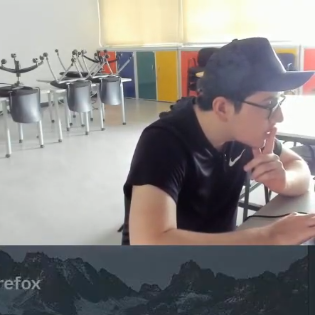
\includegraphics[width=0.8\textwidth]{resources/imagenes/Pruebas/Oscar1.png}
    \caption{Imagen de Oscar en combate}
 \end{figure}

 


\subsubsection{Cuestionario}
\begin{itemize}
    \item A pesar de lo que se mostro, le parecio confuso el sistema de debilidades y posiciones; en general las reglas describe le costo un poco entenderlas.
    \item Los jefes le parecieron algo dificiles.
    \item Las secuencia de teclas le gustaron y le parecieron en ocasiones complicadas.
    \item No le parecio muy util el acomodar a los heroes en las peleas.
    \item Le gusto la cantidad de salas a explorar.
    \item Le genero sorpresa las acciones del jefe.
    \item No le termino de convencer la ambientcaion, enemigos y diseño.
    \item Opta por merojar la colocacion de botones.
    \item Le gusta el menu de estadisticas, se le hace intuitivo.
    \item No uso mucho el mapa.
    \item Como comentario abierto menciono que seria bueno indicar mas claramente que enemigo se queire atacar.
\end{itemize}


\subsection{Usuario 2: Joshua Juarez Cruz}

Joshua es un estudiante de entre diecinueve y veintiuatro años, que dedica buen tiempo a juagar videojuegos semanalmente. Juega en cualquier 
plataforma y varia en lo que juega en generos RPG, accion-aventura, plataformas y shooters. Es preferente a los estilos visuales animados mas que realistas y le gusta la narrativa.

En RPGs le preocupa bastante la curacion de personajes y no se centra tanto en la exploracion aunque siempre le gusta ver un poco mas alla.

\subsubsection{Descripcion de prueba}

Comenzo por el tutorial y lo leyo por encima sin detenerse mucho.\\

 En el combate se llevo sorpresas divertidas por la dificultad de los time-quick-events. Inmediatamente despues de cada combate revisaba los objetos que el habian otrogado
 los comabtes. Aunque el si intento evitar lo mas posible los enfrentamientos, buscaba mas los comabte con jefes directamete. Al principio casi no le presto atencion a su vida, ni busco curacion y se enfrento al jefe
 con muy poca vida, conforme avanzo la prueba fue subiendo de nivel y encontro estrategias de hacer aatque normales con Sieg y Heracles, y hacer ataques especiales con Merlin, que fue el personaje
 que mas utlizo. Tuvo que preguntar como se equipaban los objetos. No investigo a fondo el sistema de debilidades y posiciones.\\

\begin{figure}[H]
    \centering
    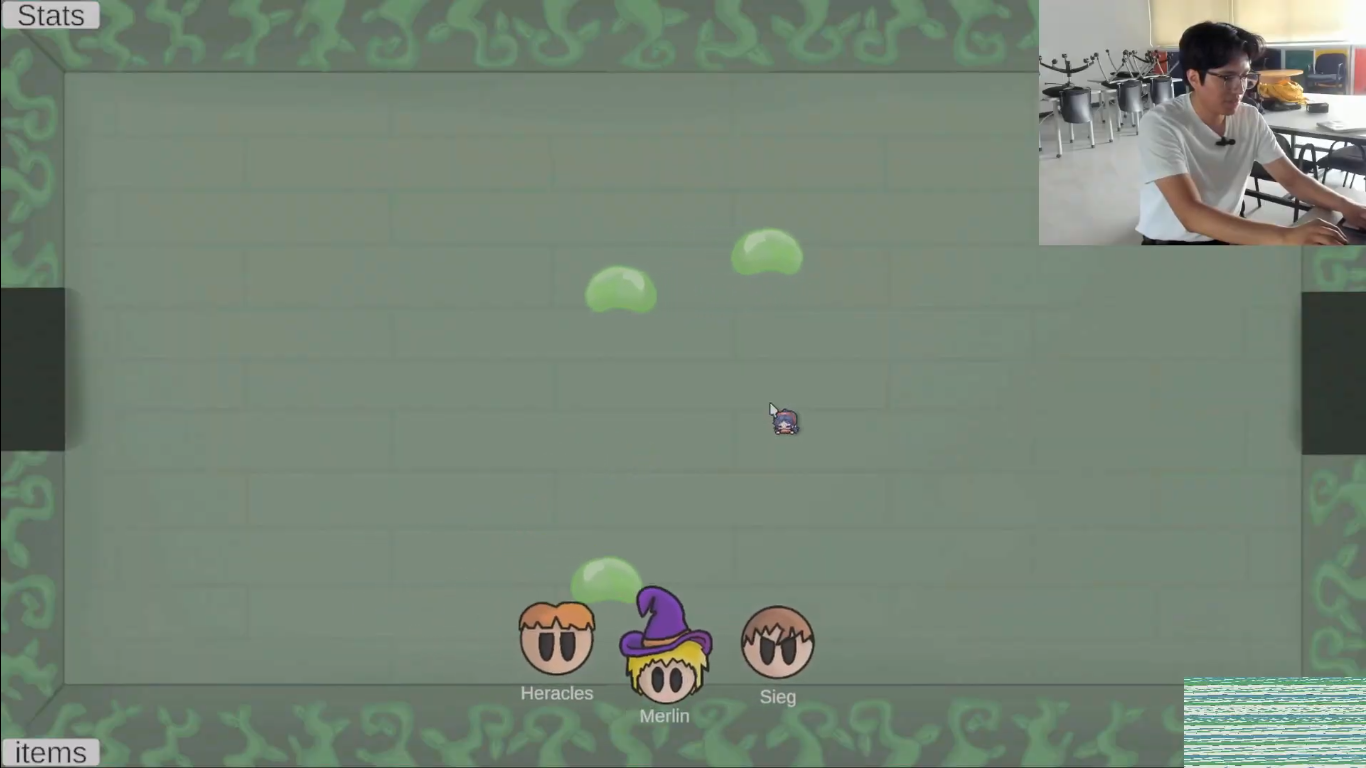
\includegraphics[width=0.8\textwidth]{resources/imagenes/Pruebas/Joshua1.png}
    \caption{Johsua esquivando enemigos}
 \end{figure}

 \begin{figure}[H]
    \centering
    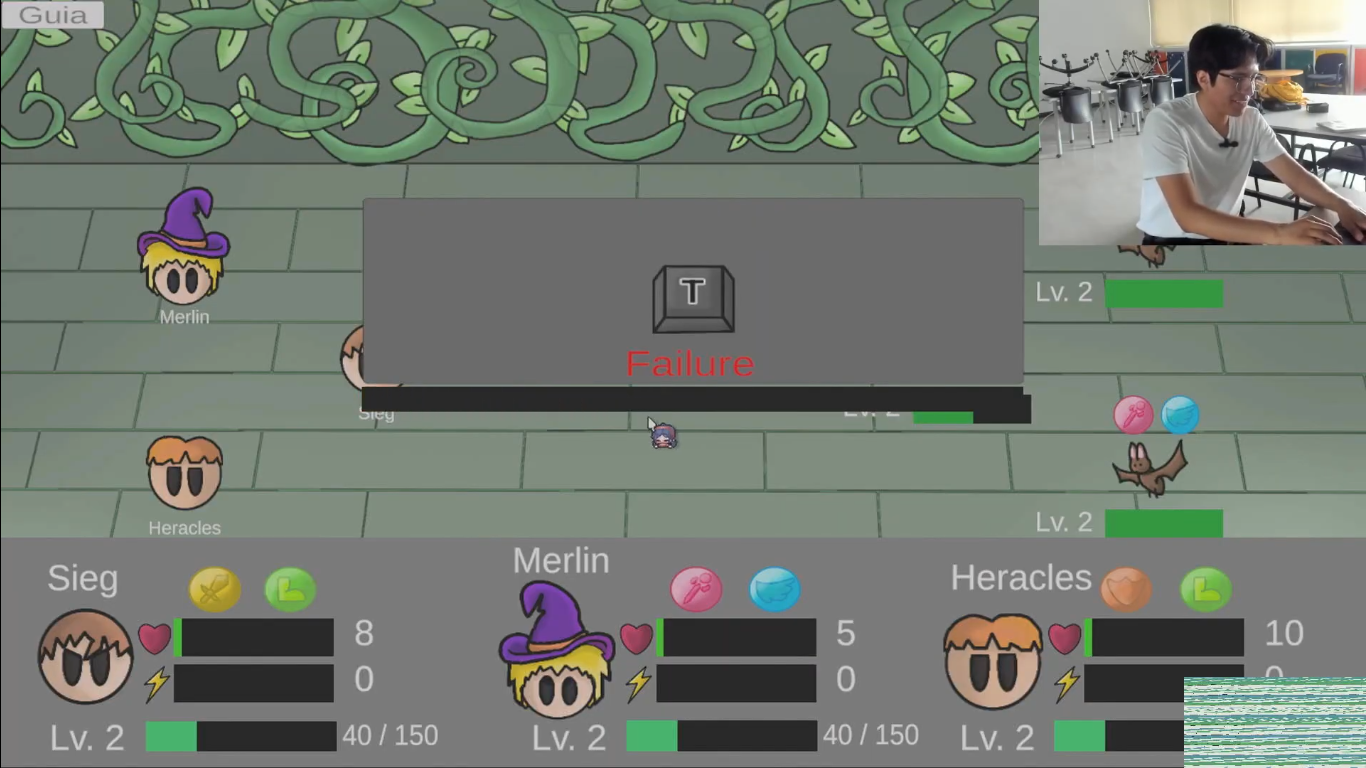
\includegraphics[width=0.8\textwidth]{resources/imagenes/Pruebas/Joshua2.png}
    \caption{Johsua reaccionando ante los time-quick-events}
 \end{figure}

\subsubsection{Cuestionario}
\begin{itemize}
    \item Le costo el comprender del sistema de debilidades y en general las reglas le costo entenderlas.
    \item Le gusto la cantidad de enemigos que habia.
    \item EL jefe le parecio dificil.
    \item Le gustaron los time-quick-events aunque en ocasiones le costaron.
    \item Muestra interes en recorrer las salas y completarlas.
    \item Se llevo pocas sorpreas.
    \item La visualizacion y el diseño le gustaron.
    \item No le comvencio la colocacion de botones. Escribio un comentario recomendando una dsitribucion que le agradaria mas.
    \item Le gusto el menu de estadisticas.
    \item No uso el mapa.
    \item Escribio un comentario para emjorar el arte y el volumen de musica.
\end{itemize}


\subsection{Usuario 3: Jessica Mayrin Garcia Lopez}

Es una estudiante de entre quince a dieciocho años, que le dedica muy pocas horas a la semana a jugar. Suele jugar en PC y dispositivos moviles modalidades
de multijugador a juegos de accion y aventura. Le gusta centrarse en mecanicas de juego con alguna historia sin demasiado contexto. Le gustan los RPG's dinamicos, aparte 
intenta buscar secretos ecplorando a fondo.

\subsubsection{Descripcion de prueba}

Leyo el tutorial muy poco, casi solo lo basico.\\

 Se le notaba divertida en los comabtes, msotraba muchas risas, y se expresaba demasiado al realizar o fallar algun time-quick-event. Variaba mas en los ataques, pero casi siempre 
 sin importar el enemigo se decatantaba por ataques especiales. No exploro el sistema de debilidades ni algun tipo de equipamiento, y de la misma manera omitio las curaciones. Se emocionaba cuando un enemigo la alcanzaba
 y mas que nada busco el combate contra el jefe. En general se desenvolvio muy flexiblemente en los time-quick-events.\\

 \begin{figure}[H]
    \centering
    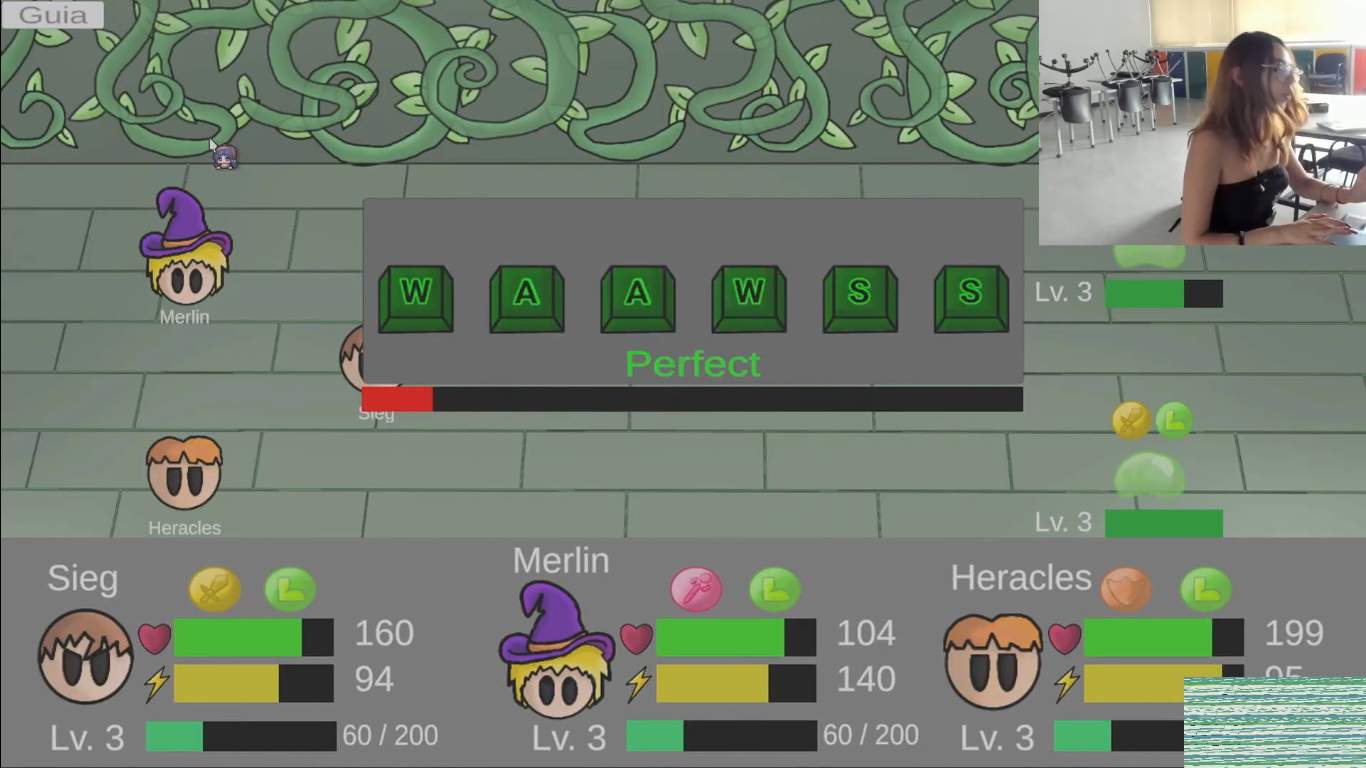
\includegraphics[width=0.8\textwidth]{resources/imagenes/Pruebas/Jessica1.png}
    \caption{Jessica reaccioando al completar un time-quick-event}
 \end{figure}

 \begin{figure}[H]
    \centering
    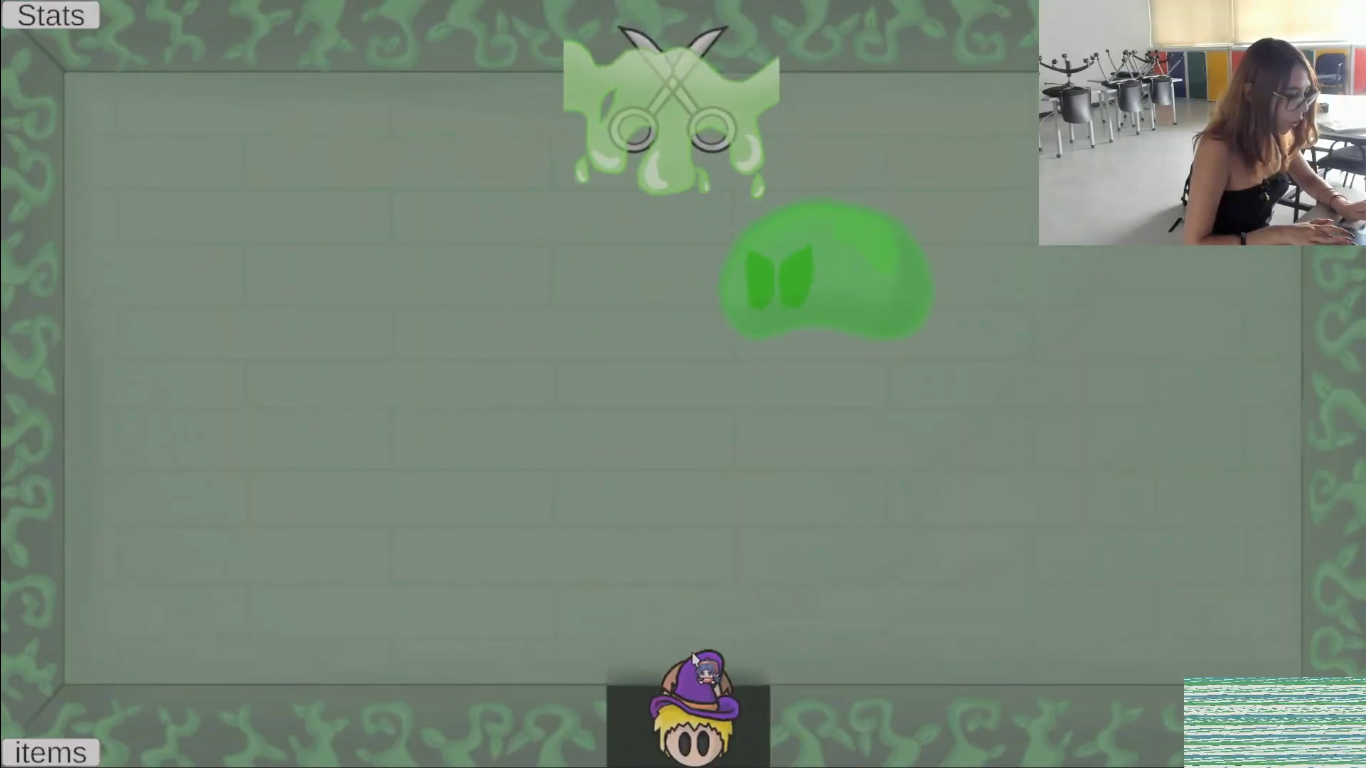
\includegraphics[width=0.8\textwidth]{resources/imagenes/Pruebas/Jessica2.png}
    \caption{Jessica sorprendida con la aparicion de un jefe}
 \end{figure}

 \subsubsection{Cuestionario}
\begin{itemize}
   \item Para ella fue claro el sistema de debilidades y las reglas muy simples.
   \item Los jefes le parecieron dificiles, pero le gusto la cantidad de enemigos por sala.
   \item Le gustaron los time-quick-events y le parecieron de dificultad media.
   \item Le interesaria explorar mas a fondo el juego.
   \item Se llevo varias sorpresas con los enemigos.
   \item Le gusto mucho y la ambientacion y el diseño.
   \item Le gusto la colocacion de los botones. 
   \item Casi no uso el mapa.
   \item En un comentario describio el juego como muy entretenido y con buena ambientacion.
\end{itemize}

\subsection{Usuario 4: Oscar Tapia Sanchez}

\subsection{Usuario 5: Oscar Tapia Sanchez}

  



\end{document}